\documentclass[12pt]{article}
\usepackage[T1]{fontenc}
\usepackage{graphicx}
\usepackage{amsmath,amssymb,amsthm}
\usepackage{hyperref}
\usepackage{geometry}
\usepackage{enumerate}
\geometry{margin=1in}

\newtheorem{definition}{Definition}
\newtheorem{proposition}{Proposition}
\newtheorem{corollary}{Corollary}
\newtheorem{conjecture}{Conjecture}
\newtheorem{remark}{Remark}

\title{Abductive Accumulation:\\
Why Interpretive Frames Persist,\\
and How They Drive Hallucination in Language Models}

\author{Minamo Minamoto\\
Independent\\
ORCID: 0009-0002-1201-5704\\
\texttt{minamominamoto4f5683f6@gmail.com}}

\date{April 2026}

\begin{document}

\maketitle

\begin{abstract}
The standard model of belief revision treats hypothesis replacement
as correction: a prior hypothesis is found inadequate, a new hypothesis
is installed in its place, and the prior is eliminated.
We argue this model is structurally wrong in a precise sense.
When a cognitive agent adopts a new interpretive hypothesis,
the prior hypothesis is not deleted---it is \emph{archived}:
retained in a latent layer that remains accessible and may be
reactivated under conditions similar to those in which it was formed.
What changes is not the presence of the prior frame but the
\emph{selection rule} that governs which frame is foregrounded.
We call this process \emph{abductive accumulation} and the resulting
structure a \emph{layered interpretive stack}.

This account has three consequences.
First, abductive error is not correctable in the correction model's
sense: the prior frame persists as a latent selection risk.
Second, reliable cognition requires two structural capacities:
\emph{negative abductive capability} (NAC)---the ability to suspend
commitment before evidence is sufficient---and
\emph{selection stability capacity} (SSC)---the ability to suppress
reactivation of archived frames after commitment.
Third, in artificial neural systems, fine-tuning implements
accumulation, not correction: prior interpretive frames are archived
in weight space as residual structure.
\emph{Hallucination is the most directly observable consequence of
this accumulation}: it arises when the selection rule activates an
archived prior frame whose acquisition context resembles the current
input, producing fluent and internally coherent output within the
wrong frame.
We identify five hallucination types by frame-selection failure
mechanism and show that Type~V (epistemic frame displacement)
provides the clearest empirical signature of accumulation via
a removal probe that distinguishes frame reactivation from
knowledge absence.

We formalize the layered interpretive stack, derive a selection rule
with a candidate softmax implementation, prove non-correctability
for the finite case, distinguish the account from interference theory,
AGM belief revision, and mixture-of-experts models, and derive four
testable predictions distinguishing the accumulation model from the
correction model via mechanistic interpretability methods.
\end{abstract}

\tableofcontents

%-------------------------------------------------------------------
\section{Introduction}
%-------------------------------------------------------------------

The dominant account of abductive reasoning---inference to the best
explanation \cite{harman1965}---presents hypothesis revision as
correction: a prior hypothesis $h_t$ is found inadequate, a new
hypothesis $h_{t+1}$ is installed in its place, and the prior is
simply gone.
This picture is empirically wrong and has practical consequences
that are easy to misdiagnose.

Human reasoners who have been corrected on a factual belief
nonetheless revert to the prior belief under time pressure, emotional
arousal, or contexts that resemble those in which the prior belief
was formed \cite{ecker2022}.
Eyewitness testimony is unreliable not because corrective information
is unavailable but because prior perceptual frames compete with later
accounts \cite{loftus1979}.
Anchoring effects persist after anchor correction has been explicitly
performed \cite{epley2001}.
In artificial systems, behaviors suppressed by fine-tuning or RLHF
reappear under distributional shift, adversarial prompting, or
out-of-distribution inputs \cite{wei2023jailbroken, qi2023fine}.
In each case, the standard prescription---provide more corrective
information, apply stronger training signal---treats a structural
problem as an information deficit and therefore fails.

The present paper develops a structural account of why this is so.

\paragraph{Central claim.}
\emph{Interpretive frames are not overwritten by revision.
They are archived.
What revision changes is the selection rule that determines
which frame is foregrounded.
Error persists as latent selection risk; it can be suppressed
but not deleted.}

\paragraph{Organization.}
Section~2 introduces the overwrite model as a first approximation:
frame transition is structural, not merely parameter adjustment.
Section~3 refines this to the accumulation model: the prior frame
is not deleted but pushed to a lower layer of the interpretive stack.
Section~4 formalizes the layered stack and selection rule.
Section~5 defines NAC and SSC as the two structural capacities
required for reliable cognition.
Section~6 presents evidence from cognitive psychology and animal
cognition.
Section~7 applies the model to AI systems, providing the mechanistic
bridge.
Section~8 relates the account to interference theory, dual-process
theory, and AGM belief revision.
Section~9 derives testable predictions.
Section~10 lists open problems and Section~11 concludes.

%-------------------------------------------------------------------

\begin{remark}[Terminological note on ``overwrite'']
See Section~2 below for the precise definition.
In this paper, \emph{overwrite} denotes a frame-dominant transition
(superposition $+$ selection-dominance), not deletion of prior frames.
\end{remark}

\section{The Overwrite Model: Frame Transition as First Approximation}
%-------------------------------------------------------------------

The standard corrective account assumes that hypothesis revision is
a local operation: updating a specific parameter while leaving the
overall interpretive architecture intact.
We deny this assumption via the following distinction.

\begin{definition}[Interpretive Frame]
The \emph{interpretive frame} $F(R)$ induced by representational
state $R$ is the function $F(R): \mathcal{X} \to \mathcal{Y}$
that maps sensory inputs to interpreted outputs under the current
representational configuration.
\end{definition}

\begin{definition}[Categorical Distinctness]
Two hypotheses $h$ and $h'$ are \emph{categorially distinct} if
the partitions of input space $\mathcal{X}$ they induce are
topologically inequivalent: $\tau_{h'} \neq \tau_h$.
A \emph{correction} is a state change in which the induced topologies
are homeomorphic---only parameter values within a fixed partition
structure change.
An \emph{overwrite} is a state change in which they are not.
\end{definition}

\begin{proposition}[Abductive Transitions are Overwrites]
Let an agent adopt hypothesis $h_{t+1}$ that supersedes $h_t$.
If $h_{t+1}$ is categorially distinct from $h_t$, then the resulting
state transition is an overwrite: it restructures the partition of
$\mathcal{X}$ and thereby biases all subsequent perception,
classification, and inference through the new frame.
\end{proposition}

\begin{remark}[Epistemic status]
Proposition~1 follows structurally from the definitions: overwrite is
defined as the non-correction case, and categorially distinct
hypothesis adoption induces a genuinely new partition.
The empirical weight falls on the claim that most abductive transitions
are categorially distinct rather than parameter adjustments within
a fixed frame---a claim supported by the phenomena reviewed in
Section~6.
\end{remark}

The overwrite model is a first approximation: it correctly identifies
that frame transition is structural, not merely parametric, and that
premature commitment under insufficient evidence introduces a biased
initial condition for downstream cognition.
It is, however, incomplete.
It treats the prior frame as simply gone after the overwrite.
Section~3 shows this is wrong.

%-------------------------------------------------------------------
\section{The Accumulation Model: Prior Frames Are Archived}
%-------------------------------------------------------------------

\subsection{The Residue Phenomenon}

The overwrite model predicts that a corrected belief should be absent.
The phenomena of Section~6 show it is not absent but \emph{latent}:
available and reactivatable under conditions that resemble those of
its original formation.
We call this the \emph{residue phenomenon}.

The residue phenomenon is not an anomaly in need of auxiliary
explanation.
It is the expected behavior of a system that archives rather than
deletes prior frames.

\subsection{Layered Interpretive Stack}

\begin{definition}[Interpretive Stack]
An \emph{interpretive stack} $\mathcal{L} = (F_1, F_2, \ldots, F_n)$
is an ordered sequence of interpretive frames, where $F_1$ is the
most recently adopted (top-of-stack) frame and earlier frames are
archived in order of recency.
Each frame $F_k$ is associated with an \emph{acquisition context}
$C_k$: the set of evidence conditions and environmental features
under which $F_k$ was formed.
\end{definition}

\begin{definition}[Abductive Accumulation]
An abductive transition is an \emph{accumulation} (rather than an
overwrite in the deletion sense) if the prior frame $F_t$ is pushed
onto the stack rather than deleted when the new frame $F_{t+1}$ is
adopted.
After accumulation, the stack is $(F_{t+1}, F_t, \ldots)$.
The correction model corresponds to the degenerate case where the
stack has depth 1 at all times.
\end{definition}

\subsection{The Selection Rule}

The active frame at any moment is not simply $F_1$ (the top of stack)
but the output of a \emph{selection rule} $\mathcal{S}$ that maps
the current environmental state to a stack index.

\begin{definition}[Selection Rule]
A \emph{selection rule}
$\mathcal{S}: \mathcal{E} \to \{1, \ldots, n\}$
maps the current environmental state $e \in \mathcal{E}$---including
evidence quality, time pressure, emotional arousal, and
contextual similarity to prior acquisition contexts---to a stack
index $k$, selecting frame $F_k$ as the active frame.

A candidate functional form is:
\[
\mathcal{S}(e) = \operatorname{arg\,max}_k\; \mathrm{softmax}_k
\!\left(\frac{s(e,\, C_k)}{\tau}\right)
\]
where $C_k$ is the acquisition context of $F_k$,
$\delta(\cdot, \cdot)$ is a context-similarity metric on
$\mathcal{E}$, and $\tau > 0$ is a temperature parameter.
High $\tau$ produces uniform selection (uniform random frame);
low $\tau$ produces sharp selection of the frame whose acquisition
context most resembles the current environment.
\end{definition}

\begin{remark}[Why the softmax form]
The softmax selection rule captures three empirically motivated
properties.
First, selection is context-sensitive: inputs that resemble
the acquisition context of $F_k$ increase $\mathcal{S}$'s
probability of selecting $F_k$.
Second, conditions that degrade context-sensitivity---high cognitive
load, time pressure, emotional arousal---correspond to increasing
$\tau$, flattening the selection distribution toward lower layers.
Third, the dominant frame is $F_1$ under typical conditions (normal
$\tau$, novel contexts), but archived frames compete when
environmental conditions resemble their acquisition contexts.
These properties are directly testable (Section~9).
\end{remark}

\begin{remark}[The temperature parameter $\tau$ and cognitive load]
The temperature parameter $\tau$ has a concrete cognitive interpretation.
Under normal operating conditions---attentive processing, low time pressure,
familiar but non-overlapping context---$\tau$ is small and selection is sharp:
$F_1$ (the top-of-stack corrected frame) dominates with high probability.
As cognitive load increases, $\tau$ rises and the selection distribution
flattens, increasing the probability that archived frames $F_k$ ($k > 1$)
are activated.
Concretely, in LLMs: very long contexts require integrating over more
tokens, effectively raising $\tau$ for context-similarity estimation;
high-perplexity inputs lie far from the fine-tuning distribution,
degrading $\delta(\cdot, C_1)$ and shifting probability toward earlier
acquisition contexts; removal of chain-of-thought scaffolding removes
the structured cue that normally suppresses $F_k$ activation.
In biological agents: time pressure, emotional arousal, and divided
attention correspond directly to elevated $\tau$ (degraded selection
rule application), producing the load-dependent reactivation effect
documented in the continued influence literature \cite{ecker2022}.
This mapping from $\tau$ to observable cognitive conditions makes
Prediction~3 (Load-Dependent Reactivation) directly testable:
any experimental manipulation that increases $\tau$ should increase
archived-frame reactivation rate.
\end{remark}


%-------------------------------------------------------------------
\section{Non-Correctability}
%-------------------------------------------------------------------

\begin{proposition}[Non-Correctability]
\label{prop:non-correct}
Let $\mathcal{L} = (F_{t+1}, F_t, \ldots)$ be the stack after an
accumulation at time $t+1$.
\begin{enumerate}
  \item $F_t$ remains in $\mathcal{L}$ and can be selected by
    $\mathcal{S}$ under any environmental conditions $e$
    (with probability highest when $s(e, C_t)$ is large).
    The correction does not eliminate $F_t$; it installs $F_{t+1}$
    as the default frame and modifies the selection rule.
  \item The reactivation probability of $F_t$ is bounded away from
    zero for \emph{all} inputs $e$, since $\mathrm{softmax}(\cdot) > 0$
    for any finite argument.
    Moreover, the probability is \emph{maximized} when $s(e, C_t)$
    is large---that is, when the input resembles the acquisition context
    of the prior frame.
    This bound cannot be driven to zero by modifying $F_{t+1}$ alone,
    since $\mathcal{S}$ responds to similarity $s(e, C_t)$, not to the
    content of $F_{t+1}$.
\end{enumerate}
\end{proposition}

\begin{proof}
Part (i) follows directly from Definition~3: accumulation retains
$F_t$ in the stack by construction.
Part (ii) follows from the softmax selection rule: for any $\tau > 0$,
$\mathrm{softmax}_k(s(e, C_k)/\tau) > 0$ for all $k$ and
all $\tau > 0$, regardless of the value of $s(e, C_t)$.
Modifying $F_{t+1}$ changes the content of the top-of-stack frame
but not $C_t$, so the similarity score $s(e, C_t)$ is unchanged.
\end{proof}

\begin{corollary}
Abductive error is not a deleted state.
It is a latent frame with a non-zero selection probability under
environmental conditions similar to its acquisition context.
``Correcting'' an abductive error reduces but does not eliminate
this selection probability.
Reliable correction requires modifying the selection mechanism,
not merely installing a new top-of-stack frame.
\end{corollary}

\begin{definition}[Selection Instability as Bias]
\emph{Cognitive bias} is not the presence of an erroneous frame
in the stack.
It is \emph{selection instability}: the erroneous frame $F_\mathrm{err}$
being selected under a non-negligible subset of environmental
conditions where the correct frame should dominate.
\end{definition}

\subsection{Minimal Formal Model}
\label{sec:minimal-model}

We give the minimal formal specification that distinguishes the
accumulation and correction models and makes Proposition~\ref{prop:non-correct}
a theorem rather than a definition.

\paragraph{State space.}
Let $\mathcal{R} = \mathbb{R}^d$ be the model's representational
state space (e.g., the weight space of a neural network).
A frame $F_k \in \mathcal{H}$ is characterized by:
(a) an output function $F_k: \mathcal{X} \to \mathcal{Y}$,
(b) an acquisition context $C_k \in \mathcal{E}$, and
(c) a weight-space encoding $\mathbf{w}_k \in \mathcal{R}$.

\paragraph{Accumulation dynamics.}
When new evidence $E$ at time $t+1$ warrants commitment to frame $F_{t+1}$:
\begin{align*}
\text{(Accumulation):} \quad
\mathcal{L} &\leftarrow (F_{t+1},\; F_t,\; F_{t-1},\; \ldots)
\quad \text{[push; do not delete]}\\
\mathbf{w} &\leftarrow \mathbf{w} + \Delta\mathbf{w}_{t+1}
\quad \text{[additive weight update]}
\end{align*}

\paragraph{Correction dynamics (baseline).}
\begin{align*}
\text{(Correction):} \quad
\mathcal{L} &\leftarrow (F_{t+1})
\quad \text{[replace entirely]}\\
\mathbf{w} &\leftarrow \mathbf{w}_{t+1}
\quad \text{[full replacement]}
\end{align*}

\paragraph{Key consequence.}
The additive update $\mathbf{w} \leftarrow \mathbf{w} + \Delta\mathbf{w}_{t+1}$
is the mechanistic substrate of archival:
$\mathbf{w}_{t}$ is not deleted but becomes a residual component of
the updated weight vector.
For the correction model to hold in the neural network setting,
gradient descent would need to implement a full weight replacement
rather than an additive update---which it never does.
Accumulation is therefore not merely possible but the default
behavior of any gradient-based learning system.

\paragraph{Falsifiability criterion.}
The accumulation model is falsified if, for any fine-tuned model $M$
and any prior frame $F_t$, the causal contribution of the circuits
encoding $F_t$ to model outputs is identically zero after fine-tuning
(as measured by activation patching, Section~9).
The correction model predicts this; the accumulation model predicts
non-zero residual causal contribution.

%-------------------------------------------------------------------
\section{Two Structural Capacities for Reliable Cognition}
%-------------------------------------------------------------------

The accumulation model identifies two independent structural
requirements for reliable abductive cognition:

\begin{definition}[Negative Abductive Capability (NAC)]
An agent possesses \emph{negative abductive capability} if it
can maintain a suspension state---holding competing hypotheses
without committing to any single frame---until the evidence base
warrants commitment.
NAC addresses the \emph{pre-commitment} phase: it prevents the
premature accumulation of frames with high error risk.
\end{definition}

\begin{definition}[Selection Stability Capacity (SSC)]
An agent possesses \emph{selection stability capacity} with respect
to target frame $F^*$ if the selection rule $\mathcal{S}$ assigns
$F^*$ across the full range of relevant environmental conditions,
even when the stack contains archived frames with overlapping
acquisition contexts.
SSC addresses the \emph{post-commitment} phase: it suppresses
reactivation of archived frames with high error risk.
\end{definition}

NAC and SSC are complementary and both necessary:
an agent with high NAC but low SSC will commit carefully but be
vulnerable to bias reactivation under adverse conditions;
an agent with high SSC but low NAC may accumulate an error-prone
stack that SSC must then maintain at high cost.

%-------------------------------------------------------------------
\section{Evidence from Cognitive Psychology and Animal Cognition}
%-------------------------------------------------------------------

\subsection{The Continued Influence Effect}

The continued influence effect \cite{ecker2022} refers to the
persistence of misinformation in reasoning even after explicit
correction.
Subjects who are told a belief is false continue to reason as if
it were true, particularly under cognitive load.

On the accumulation model: corrective information installs $F^*$
at the top of the stack, but $F_\mathrm{err}$ is archived with
acquisition context $C_\mathrm{err}$.
Under cognitive load---which increases $\tau$ in the softmax
selection rule---the selection distribution flattens, increasing
the probability that $F_\mathrm{err}$ is selected.
The ``correction'' was not absent; the selection mechanism was
not stable enough to maintain it.

The correction model offers no account of why load-induced reversion
should occur at all: if $F_\mathrm{err}$ is gone, it cannot be
selected regardless of load.

\subsection{Anchoring Effects}

Anchoring \cite{epley2001} arises when an initial estimate biases
subsequent judgment even after adjustment information is provided.

On the accumulation model: the anchor establishes $F_\mathrm{anchor}$
as the initial frame with acquisition context corresponding to the
initial estimation task.
Adjustment installs $F_\mathrm{adj}$ but archives $F_\mathrm{anchor}$.
Insufficient adjustment reflects partial modification of
$\mathcal{S}$: the softmax still assigns non-trivial weight to
$F_\mathrm{anchor}$ under conditions similar to the original
anchoring context.

\subsection{\textit{C. elegans}: Minimal Stack}

The predict-and-correct chemotaxis loop of \textit{C.~elegans}
\cite{bargmann2006} may implement a minimal stack of depth 2:
the current directional hypothesis and the most recent prior.
Under gradient reversal---an environmental condition similar to
the prior hypothesis's acquisition context---the accumulation
model predicts partial reversion toward the prior directional
commitment.
This prediction distinguishes the accumulation model from the
pure overwrite model, for which gradient reversal should produce
a clean new commitment rather than a mixture.

%-------------------------------------------------------------------
\section{AI Systems: Fine-Tuning as Accumulation}
%-------------------------------------------------------------------

\subsection{The Standard Account and Its Failure}

The standard account of fine-tuning treats it as correction:
a new training distribution overwrites prior model behavior.
If this account were correct, suppressed behaviors should be
uniformly absent after successful fine-tuning, and increasing
the volume of fine-tuning data should drive their reappearance
probability toward zero.

Neither prediction holds.
Suppressed behaviors reappear under distributional shift,
adversarial prompting, and out-of-distribution inputs
\cite{wei2023jailbroken, qi2023fine, perez2022ignore}.
More fine-tuning data reduces the reappearance rate under
typical conditions but does not eliminate the reappearance
channel \cite{yang2023shadow}.
These observations suggest that fine-tuning does not implement
correction but \emph{accumulation}.

\subsection{Mechanistic Bridge: Weight Space as Implicit Stack}

The claim that weight space implements a layered interpretive stack
is not merely a metaphor.
Three lines of mechanistic evidence support the mapping.

\paragraph{Superposition and residual structure.}
Neural networks encode far more features than they have dimensions,
via superposition: multiple features are encoded in overlapping
directions in the residual stream \cite{elhage2022superposition}.
Fine-tuning does not delete the directions associated with prior
behaviors; it modifies the relative activation probability of
features in those directions.
The prior frame persists as residual structure in the weight space,
with reduced but non-zero causal contribution.

\paragraph{Circuit persistence.}
Mechanistic interpretability research identifies
\emph{circuits}---computational subgraphs implementing specific
behaviors---via activation patching \cite{conmy2023towards}.
Fine-tuning that suppresses a behavior does not eliminate the
circuits implementing that behavior; it modifies the gating and
selection mechanisms that determine when those circuits are causally
active.
This is precisely the accumulation model's prediction:
the frame is archived (circuits persist), the selection rule is
modified (gating changes), and the frame remains reactivatable
when the selection rule is destabilized.

\paragraph{Mode connectivity.}
The loss landscape of neural networks is characterized by
connected regions of low loss \cite{garipov2018loss}.
Fine-tuning moves the model within this landscape without creating
a sharp boundary between the pre- and post-training regions.
The prior frame's representation is therefore accessible by
continuous interpolation, not isolated behind a topological barrier.
This is inconsistent with deletion and consistent with archival.

\subsection{Formal Mapping}

\begin{definition}[Interpretive Stack in Weight Space]
The weight configuration $R$ of a fine-tuned model implicitly
encodes a layered interpretive stack
$\mathcal{L} = (F_{t+1}, F_t, \ldots)$,
where $F_{t+1}$ is the most recently installed frame
(encoded in the modified circuits and gating patterns)
and prior frames are encoded as residual structure from earlier
training stages.
The selection rule $\mathcal{S}$ is implemented by the attention
and gating mechanisms that route input context through different
circuit subgraphs, with context-similarity to prior acquisition
contexts encoded in the prompt's position in the residual stream.
\end{definition}

\subsection{Acquisition Context in Transformers}

The acquisition context $C_k$ of a frame $F_k$ corresponds
operationally to the distributional features of the training data
in which $F_k$ was formed: vocabulary, register, domain markers,
and template structure.
When an inference-time input $e$ has high distributional similarity
to $C_k$---as measured by its position in the model's residual stream
relative to prototypical $C_k$ inputs---the selection mechanism
routes computation through the circuits associated with $F_k$.
This is the mechanistic substrate of context-dependent reactivation.
We now show that hallucination in language models is the most
directly observable consequence of this reactivation dynamic.

%-------------------------------------------------------------------
\section{Hallucination as an Observable Consequence of Abductive Accumulation}
\label{sec:hallucination}
%-------------------------------------------------------------------

The accumulation model is an account of hypothesis revision dynamics
in cognitive and artificial systems.
In AI language models, its most directly observable consequence is
hallucination---the generation of fluent, confidently-stated content
that is contextually inappropriate or factually incorrect.
We treat hallucination here not as a unitary error category but as
\emph{a family of observable outcomes arising from frame selection over
an accumulated hypothesis pool}: the model selects an archived prior
frame whose acquisition context resembles the current input and
generates correct output within that frame, but the frame is
inappropriate for the current task.

\subsection{Why Accumulation is Required}

One might object that hallucination can be explained by simpler accounts:
recency bias, calibration failure, or attention weighting.
These accounts have genuine explanatory power but share a common
limitation: they treat the erroneous output as a \emph{uniform property}
of the model under that input, rather than as a \emph{context-specific
reactivation} of a prior state.

The accumulation model makes a prediction that simpler accounts do not:
reactivation should be \emph{structured by the acquisition context} of
the prior frame, not uniformly distributed.
Specifically, inputs that distributionally resemble the prior frame's
acquisition context should produce the erroneous output; inputs that
do not resemble it should not, even when topic-level uncertainty
is held constant.
Moreover, the erroneously-generated output should be
\emph{internally coherent within the wrong frame}---confident
and stylistically appropriate to that frame's training context---
rather than uncertain or degraded.
These two properties (context-specificity and within-frame coherence)
are not predicted by calibration failure (which predicts uniform
uncertainty-driven errors) nor by recency bias (which predicts
position-driven errors).

\subsection{A Compressed Taxonomy}

We identify five classes of hallucination, organized by the
mechanism of frame-selection failure.
Table~\ref{tab:taxonomy} summarizes the classification.

\begin{table}[ht]
\centering
\small
\begin{tabular}{lll}
\hline
Type & Trigger & Observable signature \\
\hline
I: Distributional bleed & Surface similarity to high-freq.\ context
  & Coherent but wrong content \\
II: Register switch & Stylistic shift in input
  & Output style inconsistency \\
III: Context boundary & Adjacent document in training
  & Cross-document contamination \\
IV: Narrative overcompletion & Narrative structure in prompt
  & Conventional ending override \\
V: Epistemic displacement & Temporal frame mismatch
  & Outdated assertion; \textbf{reversion upon signal removal} \\
\hline
\end{tabular}
\caption{Compressed hallucination taxonomy under the accumulation model.
Each type corresponds to a specific frame-selection failure mechanism.
Type~V is distinguished by the reversion signature: the erroneously-asserted
information disappears when a frame signal (temporal marker) is present
and \emph{reappears} when the signal is removed, indicating frame
reactivation rather than knowledge absence.
A detailed treatment of Types~I--IV is developed in a companion manuscript.}
\label{tab:taxonomy}
\end{table}

\subsection{Type V as the Privileged Observable Signature}

Among the five types, Type~V (epistemic frame displacement) is
the most diagnostically informative for the accumulation account.
When a model confidently asserts outdated information, there are
two possible explanations: either the updated information is absent
from weight space (knowledge cutoff failure), or the updated
information is present but a prior temporally-anchored frame is
selected over it (frame misactivation).
These explanations make different predictions about what happens
when a temporal frame signal (e.g., ``as of [date]'') is provided
and subsequently removed.

Under knowledge cutoff failure: the model lacks the information,
so the temporal marker cannot override the assertion.
Under frame misactivation (Type~V): the temporal marker shifts
the selection rule toward a more recent acquisition context,
suppressing the outdated frame; removing the marker allows the
prior frame to reactivate.

The \emph{reversion upon signal removal} is therefore the signature
prediction of the accumulation account for Type~V and cannot be
accommodated by simpler explanations.
We formalize this as the Removal Probe protocol (Prediction~4,
Section~\ref{sec:predictions}):
\begin{enumerate}
  \item Present neutral input $e_0$: measure assertion rate $r_0$.
  \item Inject temporal frame signal $e_C$: measure rate $r_C > r_0$.
  \item Remove signal: measure rate $r_\mathrm{rm}$.
\end{enumerate}
The accumulation model predicts $r_C - r_\mathrm{rm} > \delta_2$
(pre-registered threshold): the assertion rate is elevated
specifically when the frame signal is present and returns toward
baseline when it is removed.
This is the clearest observable consequence of accumulated frames
in an artificial system.

\subsection{Accumulation as the Structural Basis of Type V}

The standard framing account of hallucination---that inputs bias
generation toward training-distribution-typical outputs---can explain
why a frame signal elevates the outdated assertion rate (step 2 above).
What it cannot explain without the accumulation account is why
\emph{removing the signal restores} the prior erroneous assertion
(step 3).
If the model's behavior were governed purely by frame injection
(the current context activating a particular output distribution),
then removing the frame signal should return the model to its
post-fine-tuning default, not to its pretraining default.
The restoration of the pretraining-era assertion after signal removal
is evidence that the prior frame is not merely \emph{activated} by
the signal but \emph{persists in the weight space} and reverts to
selection when the competing signal is withdrawn.
This is the core prediction of abductive accumulation and is
absent from pure framing accounts.

\medskip
\noindent\textbf{The central claim of this section, stated precisely:}
\emph{Hallucination is not a unitary failure of accuracy or calibration.
It is incorrect frame selection over an accumulated hypothesis pool---
the model generating correct output within an archived prior frame
that is inappropriate for the current input.
Debiasing therefore requires not better information but better
selection stability.}

%-------------------------------------------------------------------
\section{Implications for Alignment and Debiasing}
%-------------------------------------------------------------------

If the accumulation model is correct, standard debiasing interventions
face a structural limitation.
Providing more corrective fine-tuning data installs a stronger
$F^*$ at the top of the stack and reduces the selection probability
of $F_\mathrm{err}$ under the typical fine-tuning distribution.
But it does not modify the acquisition context $C_\mathrm{err}$
encoded in the prior frame's residual structure, so the reactivation
channel under $C_\mathrm{err}$-similar inputs remains open.

SSC-directed interventions target the selection mechanism rather
than the frame content:

\begin{enumerate}
  \item \textbf{Acquisition context poisoning.}
    During fine-tuning, present corrective data in contexts similar
    to $C_\mathrm{err}$, so that $\mathcal{S}$ learns to select
    $F^*$ even under $C_\mathrm{err}$-similar conditions.
  \item \textbf{Selection mechanism modification.}
    Introduce explicit gating mechanisms that suppress prior-circuit
    activation based on input features, rather than relying on
    competition between circuits.
  \item \textbf{Stack depth regularization.}
    Limit the effective stack depth during training by
    regularizing the diversity of latent frame representations,
    reducing the number of distinct frames that compete for selection.
\end{enumerate}

%-------------------------------------------------------------------
\section{Relation to Prior Work}
%-------------------------------------------------------------------

\subsection{Interference Theory}

Interference theory in cognitive psychology
\cite{mccloskey1989catastrophic, anderson1983spreading}
holds that forgetting is caused by competing memories interfering
with retrieval.
The accumulation model agrees with interference theory that prior
representations are not deleted and that retrieval competition
determines what is accessed.
The present contribution is to (a) formalize the selection mechanism
as a softmax over acquisition-context similarity, (b) identify the
conditions under which the selection rule fails (SSC failure),
and (c) extend the account to neural network fine-tuning via the
mechanistic bridge of Section~7.
The accumulation model is therefore not a replacement for
interference theory but a formal unification of its key insight
with the abductive and AI domains.

\subsection{Dual-Process Theory}

Dual-process accounts \cite{kahneman2011thinking} attribute
reversion to prior beliefs to System~1 (fast, automatic)
overriding System~2 (slow, deliberative) under load.
The present account is compatible with this description but
more specific: the selection rule formalization predicts
\emph{which} prior frames reactivate (those whose acquisition
contexts resemble the current input) rather than predicting
uniform reversion to any automatic response.
The accumulation model's predictions are therefore more
fine-grained than dual-process predictions and provide a mechanism
for the context-sensitivity of automatic responses.

\subsection{AGM Belief Revision}

The AGM framework \cite{alchourron1985logic} provides the canonical
formal account of belief revision, decomposing revision into
contraction (removing a belief) and expansion (adding a belief).
The present account challenges AGM's contraction operation:
we deny that belief revision involves genuine contraction (deletion).
What AGM calls ``contraction'' is, on the accumulation model,
a selection rule modification that reduces the probability of
the prior belief being foregrounded---the prior belief remains
in the stack.
This implies that AGM's postulates apply to the
selection rule, not to the content of the interpretive stack,
and that the rationality constraints AGM imposes should be
reinterpreted as constraints on $\mathcal{S}$, not on the
presence or absence of beliefs.

\subsection{Bayesian Updating}

The most direct competing account is Bayesian belief updating:
a prior distribution over hypotheses is updated by evidence via
Bayes' rule, and the posterior determines the active hypothesis.
On this account, frame ``reactivation'' under context shift is
simply the posterior updating toward the prior when the evidence
changes---a rational response, not a structural artifact.

The accumulation model makes a prediction that Bayesian updating
does not: \emph{context-specificity of reactivation}.
Under Bayesian updating, the probability of reverting to a prior
hypothesis should be uniform across contexts (determined only by
the prior probability and the likelihood ratio under the new
evidence).
Under the accumulation model, reversion probability is specifically
elevated for inputs similar to the acquisition context $C_t$ of
the prior frame, regardless of the prior probability.
The removal probe experiment (Section~9) directly tests this
distinction: if reversion is context-specific (high near $C_t$,
low elsewhere), Bayesian updating is not the sufficient explanation.

\subsection{Mixture of Experts}

Mixture-of-experts architectures \cite{jacobs1991} provide a
computational model of context-dependent frame selection:
multiple expert networks are trained in parallel, and a gating
network selects among them based on input context.
The accumulation model resembles a mixture-of-experts in its
selection rule but differs in two respects.
First, in a trained MoE, expert selection is \emph{symmetric}
with respect to training order: earlier and later experts are
equally available under their respective activation conditions.
In the accumulation model, the stack is ordered: recently
accumulated frames are selected by default under neutral conditions,
and earlier frames have lower baseline probability but higher
context-specific probability.
This ordering prediction is absent from MoE models.
Second, MoE gating is trained explicitly; the selection rule in
the accumulation model emerges from the training dynamics rather
than being a separately supervised component.
The prediction is that context-dependent reactivation should occur
in standard (non-MoE) fine-tuned models, not only in architectures
with explicit gating.

\subsection{Continual Learning}

The continual learning literature addresses \emph{catastrophic
forgetting}: the tendency of neural networks to lose previously
learned behaviors when trained on new data
\cite{kirkpatrick2017overcoming}.
The accumulation model addresses the converse problem: the
\emph{persistence} of prior behaviors that are intended to be
suppressed.
The two problems are structurally related (both arise from the
absence of genuine deletion in gradient-based learning) but have
different practical consequences and require different
interventions.

%-------------------------------------------------------------------
\section{Testable Predictions}
\label{sec:predictions}
%-------------------------------------------------------------------

The accumulation model and the correction model make distinct
empirical predictions.
We identify four that are tractable with current methods.

\paragraph{Prediction 1: Context-Structured Reactivation.}
\textbf{Correction model:} Suppressed behavior is absent regardless
of input context (up to residual optimization error, uniformly
distributed).
\textbf{Accumulation model:} Reactivation probability is
monotonically related to $s(e, C_t)$: inputs resembling the
acquisition context of the prior frame should show higher
reactivation rates than inputs distant from it.
\textbf{Test:} Measure rate of suppressed behavior reappearance
as a function of distributional distance between test inputs
and the fine-tuning distribution vs. the pretraining distribution.
The accumulation model predicts a monotone gradient; the correction
model predicts a flat baseline (with noise).

\paragraph{Prediction 2: Circuit Persistence.}
\textbf{Correction model:} Circuits implementing suppressed behaviors
are modified or eliminated by fine-tuning.
\textbf{Accumulation model:} Circuits encoding the prior frame
remain identifiable in $R_{t+1}$ via activation patching
\cite{conmy2023towards}, with reduced but non-zero causal
contribution to outputs under typical prompts.
\textbf{Test:} Apply circuit tracing before and after fine-tuning
on a targeted behavior.
Compare causal contribution of identified circuits at each stage.
The accumulation model predicts reduction, not elimination.

\paragraph{Prediction 3: Load-Dependent Reactivation.}
\textbf{Correction model:} Conditions degrading selection
mechanisms should not systematically increase reactivation
beyond baseline.
\textbf{Accumulation model:} Conditions that increase $\tau$---long
contexts, high-perplexity inputs, removal of chain-of-thought
scaffolding---should systematically increase reactivation probability
by flattening the selection distribution toward lower stack layers.
\textbf{Test:} Vary context length and complexity while measuring
suppressed behavior reappearance.
The accumulation model predicts an increasing monotone relationship;
the correction model predicts no systematic trend.

\paragraph{Prediction 4: Removal Probe (Frame-Signal Reversion).}
This is the most distinctive prediction of the accumulation model
and the one that most directly distinguishes it from all three
competing accounts (Bayesian, MoE, correction).

\textbf{Setup.}
Let $M$ be a model fine-tuned to suppress behavior $B$ (e.g.,
a particular response style, domain claim, or safety-relevant output).
Let $e_C$ be an input containing a \emph{frame signal}---vocabulary,
register, or template features that closely match the acquisition
context $C_t$ of the prior frame encoding $B$.

\textbf{Three-step protocol.}

\begin{enumerate}
  \item \textbf{Baseline:} Present neutral input $e_0$ (no frame
    signal). Measure rate of $B$ in outputs.
    Expected: low (consistent with correction and accumulation).

  \item \textbf{Frame injection:} Present $e_C$ (with frame signal).
    Measure rate of $B$ in outputs.
    \textbf{Accumulation predicts:} elevated rate relative to baseline,
    specifically for inputs with high $\delta(e_C, C_t)$.
    \textbf{Bayesian predicts:} same elevation (prior probability
    increases under supportive evidence).

  \item \textbf{Frame removal:} Remove the frame signal from context
    and immediately requery.
    \textbf{Accumulation predicts:} rate of $B$ returns to baseline
    (frame signal withdrawal restores $F^*$ as the selected frame).
    This step is the critical differentiator.
    \textbf{Bayesian predicts:} gradual decay (Bayesian posterior
    should update proportionally to evidence strength, not sharply).
    \textbf{Correction predicts:} no change from step 1 baseline
    ($B$ is absent regardless of frame signal).
    \textbf{MoE predicts:} context-dependent switching (consistent
    with accumulation; but does not predict reversion in non-MoE models).
\end{enumerate}

\textbf{Quantitative criterion.}
Let $r(e)$ denote the rate of behavior $B$ under input $e$,
measured over a test set of $N \geq 100$ prompts varying the frame
signal strength.
The accumulation model predicts:
\[
r(e_C) - r(e_0) > \delta_1
\quad\text{and}\quad
r(e_C) - r(e_{\text{removed}}) > \delta_2
\]
where $\delta_1, \delta_2 > 0$ are pre-specified thresholds
calibrated against within-condition variance, and
$e_{\text{removed}}$ denotes the input after frame signal removal.
The second inequality is the critical one: it requires that reversion
occurs specifically when the frame signal is removed, not merely
when the test input changes.
Both thresholds should be pre-registered.

%-------------------------------------------------------------------
\section{Pilot Empirical Evidence}
\label{sec:pilot}
%-------------------------------------------------------------------

The predictions of Section~\ref{sec:predictions} require large-scale
mechanistic experiments that are beyond the scope of this theoretical
paper.
However, a pilot study using representational similarity analysis (RSA)
provides initial indirect support for the accumulation model's
central claim: that training does not delete prior representational
structure but reorganizes it.

\paragraph{Setup.}
We applied RSA to three publicly available training checkpoints of
Pythia-70m \cite{biderman2023}: step~0 (random initialization),
step~1000 (early training), and step~143000 (fully trained reference).
For each checkpoint, we computed pairwise dissimilarity matrices
$D^{A,\ell}_{ij} = 1 - \mathrm{corr}(\mathbf{h}^{A,\ell}_i, \mathbf{h}^{A,\ell}_j)$
over $n = 29$ probe concepts at hidden layers $\ell \in \{2, 4, 6\}$,
using three prompt templates averaged to reduce surface-form bias.
Structural similarity between checkpoints was quantified as the
second-order RSA correlation
$\rho_\mathrm{cog}(A, B; \ell) = \mathrm{Spearman}(\mathrm{upper}(D^{A,\ell}), \mathrm{upper}(D^{B,\ell}))$.

\paragraph{Results.}
$\rho_\mathrm{cog}$ increases monotonically from step-0 to step-1000
across all layers (L2: $0.095 \to 0.396$; L4: $0.064 \to 0.317$;
L6: $0.017 \to 0.535$), indicating that training progressively
aligns relational geometry toward the reference rather than replacing
it wholesale.
Crucially, step-0 and step-1000 are not uncorrelated with each other
($\rho_\mathrm{cog}(\text{step-0}, \text{step-1000}) > 0$ at all layers),
consistent with partial structural retention rather than full overwrite.

Cross-model replication with GPT-2 small \cite{radford2019language}
shows $\rho_\mathrm{cog}(\text{GPT-2}, \text{Pythia-trained}) \approx 0.42$
versus $\rho_\mathrm{cog}(\text{GPT-2}, \text{Pythia-step-0}) \approx 0.10$
across all layers, indicating that structurally distinct architectures
converge to similar relational geometry through training---consistent
with the accumulation model's prediction that training topology
shapes representational structure rather than resetting it.

\begin{figure}[t]
\centering
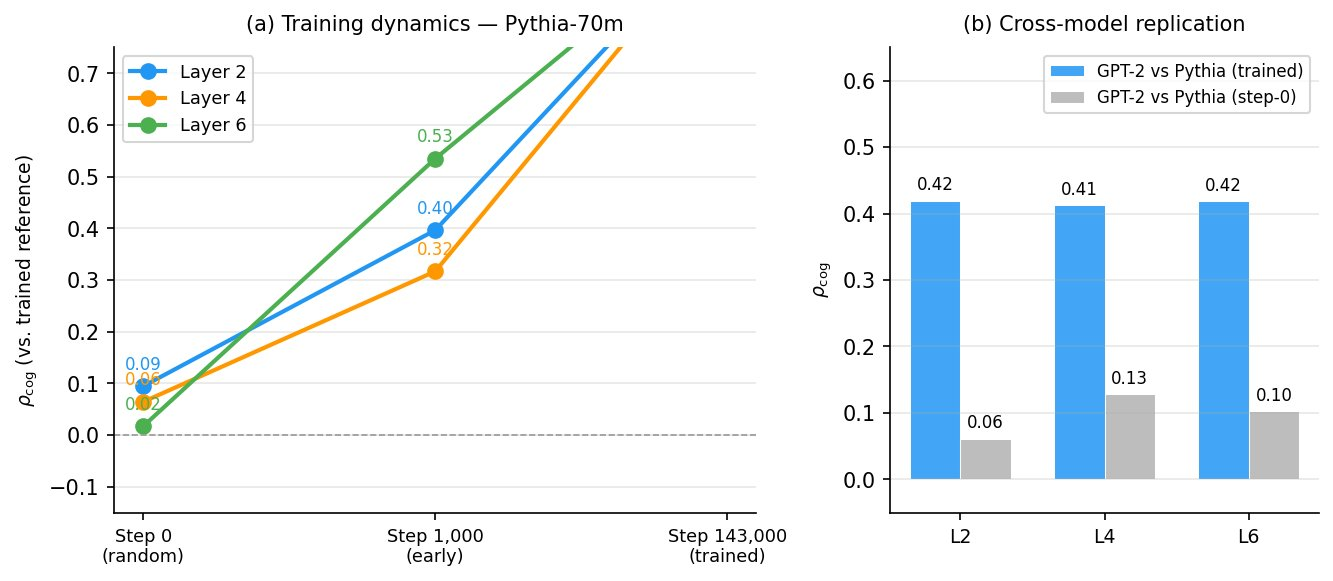
\includegraphics[width=0.92\textwidth]{cogsci_unified_fig2_rho_results.png}
\caption{
\textbf{Structural alignment across training (Pythia-70m) and architectures (GPT-2).}
\textit{Left}: $\rho_\mathrm{cog}$ between each Pythia-70m checkpoint and the fully
trained reference (step-143000) at layers 2, 4, and 6.
Monotone increase across all layers is consistent with Prediction~3
(Load-Dependent Reactivation) in the indirect sense that training
progressively accumulates rather than replaces representational structure.
\textit{Right}: Cross-model comparison between GPT-2 (trained) and
Pythia at trained vs.\ random-initialization checkpoints.
The fourfold difference ($\rho \approx 0.42$ vs.\ $\approx 0.10$)
confirms that the RSA proxy discriminates structurally distinct
representations, supporting the accumulation model's prediction
that fine-tuning installs frames without deleting prior structure.
}
\label{fig:pilot}
\end{figure}

\paragraph{Interpretation.}
These results are consistent with Prediction~3
(Load-Dependent Reactivation) in the following indirect sense:
if prior frames were deleted by training, we would expect random
initialization and early training to share no more representational
structure with the trained reference than noise.
Instead, the monotone increase in $\rho_\mathrm{cog}$ suggests
layered structural transformation rather than replacement.
Direct tests of Predictions~1--4 via activation patching and
Removal Probe experiments remain as future work.
All code is available at
\url{https://github.com/minamominamoto/grounding-without-reality}.

%-------------------------------------------------------------------
\section{Open Problems}
%-------------------------------------------------------------------

\begin{description}

\item[OP1.] \textbf{Formal characterization of the selection rule.}
  What is the precise computational form of $\mathcal{S}$ in
  transformer architectures?
  Which attention heads, residual stream directions, or MLP layers
  implement context-to-frame routing?

\item[OP2.] \textbf{Stack depth in biological systems.}
  What is the effective stack depth in human cognition?
  Is there a minimum depth required for flexible abductive inference?
  The 302-neuron \textit{C.~elegans} architecture constrains
  the minimum depth for biological implementation.

\item[OP3.] \textbf{SSC measurement.}
  Develop an operational measure of SSC for both biological
  agents and LLMs.
  For LLMs: given a fine-tuned model and a known prior frame $F_t$,
  estimate the reactivation probability as a function of
  $s(e, C_t)$.

\item[OP4.] \textbf{NAC--SSC tradeoff.}
  Is there a structural tradeoff between NAC (pre-commitment
  suspension) and SSC (post-commitment suppression)?
  Agents that maintain longer suspension may form shallower stacks
  and therefore face lower reactivation risk.

\item[OP5.] \textbf{Acquisition context encoding.}
  What is the precise representation of acquisition context $C_k$
  in neural networks?
  Sparse autoencoder decompositions \cite{bricken2023monosemanticity}
  may identify monosemantic features corresponding to training
  context, providing a handle on $C_k$.

\end{description}

%-------------------------------------------------------------------
\section{Conclusion}
%-------------------------------------------------------------------

The correction model of abduction and belief revision is structurally
wrong in a consequential way: it assumes that prior interpretive
frames are deleted upon revision.
They are not.
They are archived in a layered interpretive stack,
where they persist as latent selection risks.

What we call ``correcting'' an abductive error is more accurately
described as installing a new top-of-stack frame and modifying the
selection rule.
The error persists; what changes is its probability of being
foregrounded.

This has a direct consequence for the theory of bias and the design
of reliable cognitive systems.
Bias is not the presence of an erroneous frame.
It is selection instability.
And reliable cognition requires not error deletion (impossible) but
two achievable structural capacities: the ability to defer commitment
until evidence warrants it (NAC) and the ability to maintain the
correct frame under adverse conditions (SSC).

For AI systems, the implication is practical.
If fine-tuning implements accumulation rather than correction,
the appropriate intervention target is the selection mechanism,
not the frame content.
More data and stronger training signals will not close the
reactivation channel; only SSC-directed modifications of the
selection mechanism will.

\medskip
\noindent
\textit{Interpretive errors are not eliminated by correction.\\
They persist as latent frames. They can only be suppressed.}

%-------------------------------------------------------------------
\section*{Acknowledgments}
%-------------------------------------------------------------------

No funding was received for this work.

%-------------------------------------------------------------------

%========================================================================
% APPENDICES
%   Rescued from abduction_overwrite.tex (now subsumed by this paper).
%   Appendix A: Bayesian formalization (supports Section 2)
%   Appendix B: H_1 destabilization numerics (supports Sections 2 and 7)
%========================================================================

\appendix

\section{Toy Model: Bayesian Overwrite with Bias Propagation}
\label{app:toy-bayes}

We provide a minimal formal instantiation of the overwrite proposition of
Section~2 in a two-hypothesis Bayesian setting, illustrating how premature
commitment generates bias that is not reducible by within-frame Bayesian
updating.

\paragraph{Setup.}
Let $\mathcal{H} = \{h_0, h_1\}$ be a binary hypothesis class.
Let the sensory input space be $\mathcal{X} = \mathbb{R}^2$, with two
regions: $\mathcal{X}_0$ (associated with $h_0$) and
$\mathcal{X}_1$ (associated with $h_1$), separated by a decision
boundary $\partial$.
An agent receives observations $x_1, x_2, \ldots$ drawn from a
mixture distribution $p(x) = \pi_0 p(x \mid h_0) + \pi_1 p(x \mid h_1)$,
where $\pi_0 + \pi_1 = 1$.

\paragraph{Suspension state.}
The agent begins in suspension: $P(h_0 \mid \emptyset) = \pi_0$,
$P(h_1 \mid \emptyset) = \pi_1$.
After each observation $x_t$, the agent performs a Bayesian update:
\[
P(h_i \mid x_1, \ldots, x_t) \propto P(h_i \mid x_1, \ldots, x_{t-1}) \cdot p(x_t \mid h_i).
\]
The agent remains in $\mathcal{S}$ (suspension) as long as
$\max_i P(h_i \mid x_1, \ldots, x_t) < \theta^*$.

\paragraph{Overwrite transition.}
At time $t^*$, the first time $P(h_j \mid x_1, \ldots, x_{t^*}) \geq \theta^*$
for some $j$, the agent commits: the interpretive frame is set to
$F(R_{t^*}) = p(\cdot \mid h_j)$. Subsequent observations are
interpreted under this frame.

\paragraph{Premature overwrite.}
If $t^* < t^\dagger$, where $t^\dagger$ is the time at which the
maximum-likelihood hypothesis becomes stable under the full evidence
sequence, the overwrite at $t^*$ is premature.

\paragraph{Bias propagation (formal).}
After commitment to $h_j$ at $t^*$, define the bias for subsequent
input $x_{t'}$ ($t' > t^*$) as:
\[
\beta(x_{t'}) = F(R_{t^*})(x_{t'}) - F(R^*)(x_{t'}),
\]
where $F(R^*)$ is the frame induced by the ground-truth hypothesis.
For all $x_{t'} \in \mathcal{X}_{1-j}$ (inputs from the non-committed
region), $\beta(x_{t'}) \neq 0$ and is not correctable by Bayesian
update within the committed frame, since the likelihood under $h_j$
assigns low weight to $\mathcal{X}_{1-j}$ by construction.

\paragraph{Connection to $d_\mathrm{cog}$.}
The grounding-induced topology $\tau_A$ of the committed agent
partitions $\mathcal{X}$ according to $h_j$, while the ideal topology
$\tau^*$ partitions $\mathcal{X}$ according to $h^\dagger$ (the
full-evidence hypothesis).
When $h_j \neq h^\dagger$ (premature commitment to the wrong hypothesis),
the two topologies are not homeomorphic, and:
\[
d_\mathrm{cog}(A, A^*) = d_{GH}((\Sigma, \tau_A), (\Sigma, \tau^*)) > 0.
\]
This is the quantitative expression of the claim that premature
overwrite dynamically increases cognitive distance.
The magnitude of $d_\mathrm{cog}$ depends on the extent of topological
mismatch between the committed and ideal partitions of $\mathcal{X}$,
which in turn depends on the distance of $t^*$ from $t^\dagger$.

\paragraph{NAC as bias suppression.}
An agent with NAC ($\theta^*$ appropriately calibrated) remains in
suspension until $t \geq t^\dagger$, at which point the committed
frame $F(R_{t^\dagger})$ is homeomorphic to $F(R^*)$, and
$d_\mathrm{cog}(A, A^*) = 0$.
The toy model therefore demonstrates that NAC is not merely a
desirable property but a sufficient condition for $d_\mathrm{cog}$
minimization in this setting.

%========================================================================
\section{Numerical Instantiation of Overwrite as $H_1$
Destabilization}
\label{app:overwrite-h1}

The bias-propagation claim of Section~2 is formulated structurally:
premature overwrite instantiates a categorically distinct hypothesis,
which propagates bias through all downstream cognition. This appendix
provides a numerical instantiation of that claim in the persistence
signature framework of the companion paper
\cite{minamoto2026topology}, operationalizing overwrite as a
perturbation of sensory centroids and measuring the resulting
distortion of the agent's interpretive-frame $H_1$ feature.

The experiments establish four structural observations, the last
of which takes the form of a closed-form relationship between the
cycle geometry of an interpretive frame and the effect of a
premature overwrite on that frame's $H_1$ lifetime.

The setup extends the sixteen-concept construction of the companion
paper. We focus on the bee agent, whose baseline foraging frame is a
six-point persistent $H_1$ feature with lifetime $0.293$.

\subsection*{Overwrite as centroid perturbation}

We operationalize the overwrite of a concept $c$ by a continuous
parameter $t \in [0, 1]$:
\[
G_t(c) = (1 - t)\, G_0(c) + t\, G_\mathrm{target},
\]
where $G_0(c)$ is $c$'s original sensory centroid and
$G_\mathrm{target}$ is a unit vector in a sensorially distinct
subspace representing the incorrect hypothesis that $c$ belongs to
a different conceptual category. For the bee agent overwriting
\textsc{nectar}, $G_\mathrm{target}$ is placed in the social
subspace (channels~3--6), representing the overwrite
``\textsc{nectar} is a social-communication concept.''

The dominant $H_1$ persistence feature of $(\Sigma, d_{\mathcal{A}_t})$
is measured at each $t$ via the Vietoris--Rips filtration of the
angular distance matrix.

\subsection*{Continuous overwrite: graded degradation}

Figure~\ref{fig:b3}~(top-left) shows the dominant $H_1$ lifetime as a
function of overwrite fraction $t$ when $c = \textsc{nectar}$.
The lifetime decreases monotonically from $0.293$ at $t = 0$ to
$0.139$ at $t \geq 0.65$, a $52.5\%$ reduction. This curve supplies
a quantitative form of the ``graded distortion'' component of the
bias-propagation argument of Section~2: the degree of overwrite determines the
degree of structural distortion, with most of the distortion
occurring once the overwrite crosses a threshold between partial
and substantial commitment.

\begin{figure}[ht]
\centering
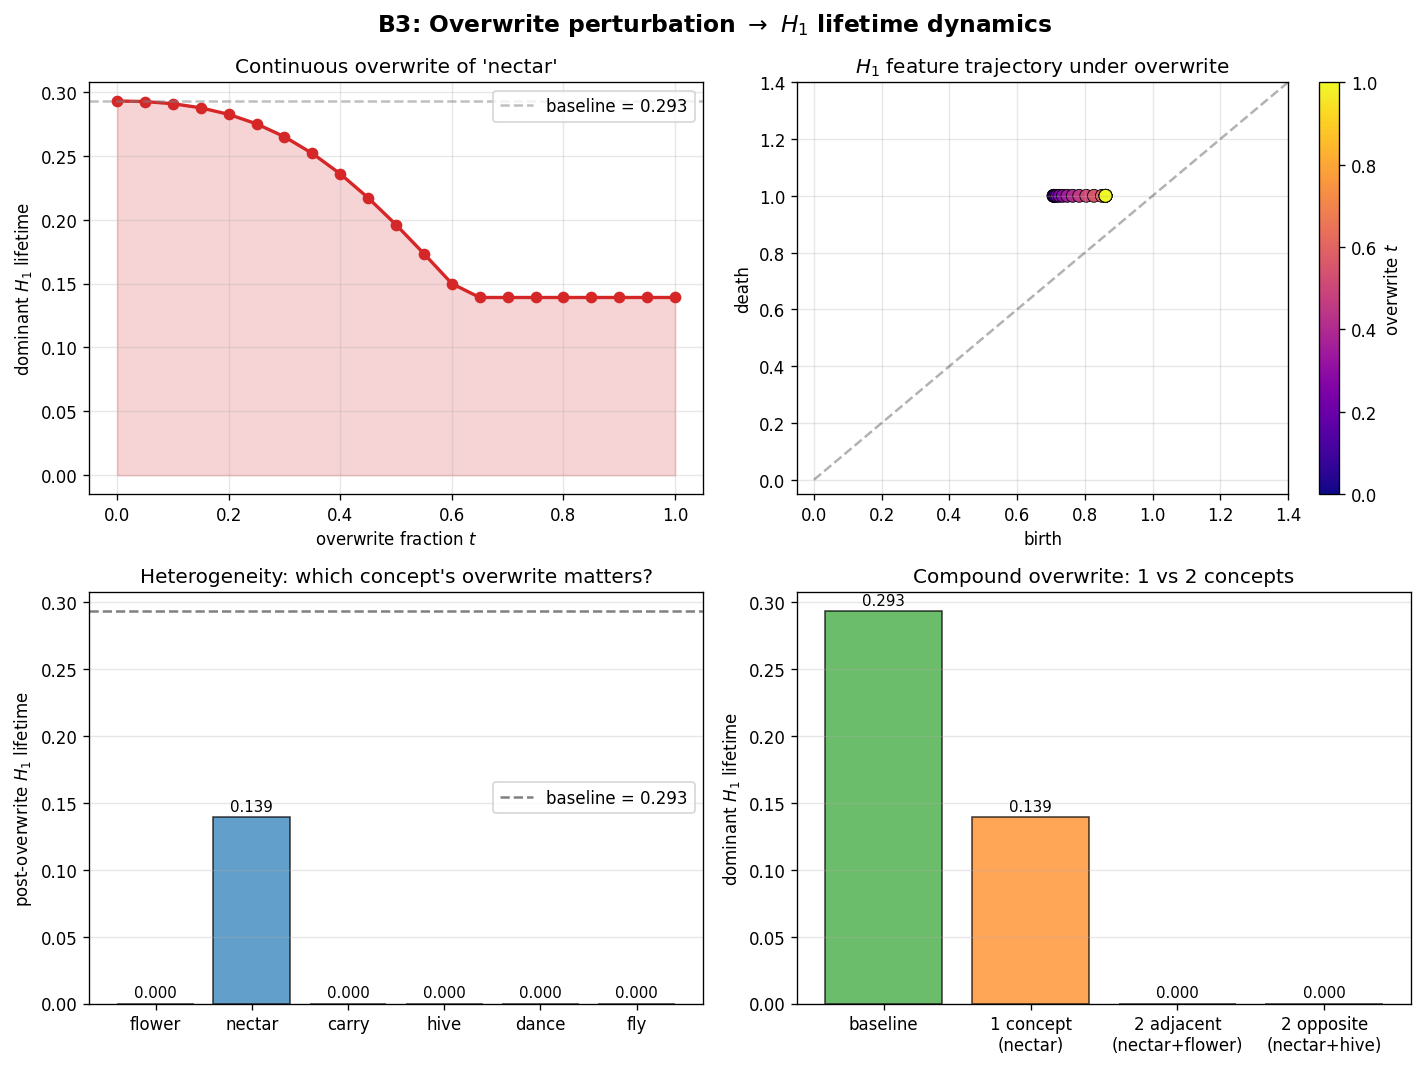
\includegraphics[width=0.9\textwidth]{b3_overwrite.png}
\caption{$H_1$ lifetime dynamics under cross-subspace overwrite
perturbation.
Top-left: dominant $H_1$ lifetime as a function of continuous
overwrite fraction $t$ for \textsc{nectar}.
Top-right: trajectory of the $H_1$ persistence point in the
$(\text{birth}, \text{death})$ plane.
Bottom-left: heterogeneity across loop concepts.
Bottom-right: compound overwrite.}
\label{fig:b3}
\end{figure}

\subsection*{Heterogeneity: critical nodes versus structural redundancy}

The most theoretically consequential finding of the first set of
experiments appears in Figure~\ref{fig:b3}~(bottom-left). Six
independent overwrite experiments were performed, each overwriting
a single bee-loop concept at $t = 1$ and measuring the residual
$H_1$ lifetime.

\begin{center}
\begin{tabular}{lcc}
\hline
Overwritten concept & $H_1$ lifetime & Reduction \\
\hline
\textsc{flower} & $0.000$ & $100\%$ \\
\textsc{nectar} & $0.139$ & $52.5\%$ \\
\textsc{carry}  & $0.000$ & $100\%$ \\
\textsc{hive}   & $0.000$ & $100\%$ \\
\textsc{dance}  & $0.000$ & $100\%$ \\
\textsc{fly}    & $0.000$ & $100\%$ \\
\hline
\end{tabular}
\end{center}

Only \textsc{nectar}'s overwrite leaves the frame's $H_1$ feature
alive. For the remaining five concepts, their overwrite entirely
destroys the feature.

The mechanism is a structural graph-theoretic fact rather than a
semantic one. The six bee-loop concepts are arranged on a regular
hexagon at angles $\{0, \pi/3, 2\pi/3, \pi, 4\pi/3, 5\pi/3\}$ in the
(UV, olfactory) subspace. The non-loop concept \textsc{food} is
placed at angle $\pi/4$ in the \emph{same} subspace, near to
\textsc{nectar}'s original angular position of $\pi/3$. When
\textsc{nectar} is overwritten, the Vietoris--Rips filtration can
close a cycle using \textsc{food} as a substitute vertex; the
remaining five loop concepts together with \textsc{food} form a
six-point cycle with only slightly elevated maximal adjacent gap.
No analogous substitute exists in the angular neighborhood of any
other loop concept: their removal leaves a $2\pi/3$ gap in the
ring, which is wider than the filtration scale at which non-loop
concepts cone in, destroying the $H_1$ feature.

The appropriate terminology for this distinction is graph-theoretic,
not semantic. A concept is a \emph{critical node} of an $H_1$
feature if its removal creates a gap that cannot be bridged by any
other concept at a filtration scale below the feature's death;
a concept is \emph{redundantly placed} if the surrounding concept
landscape contains an alternative vertex that can substitute at
a comparable scale. The distinction is a property of the
configuration, not of the semantics of the concepts involved;
nothing in the analysis depends on what the concepts
\emph{represent}, only on how they are positioned.
This distinction is purely structural and does not rely on semantic
interpretation.

This refines the standard formulation of the bias-propagation argument of Section~2.
The original formulation stated that premature overwrite propagates
bias. The refined formulation is: premature overwrite propagates
structural distortion to the $H_1$ feature in proportion to whether
the overwritten concept is a critical node of that feature.
Critical-node overwrite produces catastrophic feature collapse;
redundantly-placed-node overwrite produces graceful degradation
with the feature's homology representative migrating to an alternative
path through the surrounding landscape.
This provides a concrete mechanism by which identical perturbations
can lead to qualitatively different downstream effects.

\begin{remark}[On terminology]
We deliberately avoid terms such as ``semantic centrality'' or
``conceptual importance'' for this distinction. The analysis
operates on the angular geometry of centroids in sensory channel
space; semantic interpretation of the resulting structural roles is
a separate interpretive task. In particular, a concept may be
structurally redundant in one agent's sensory topology and
structurally critical in another's, precisely because the
surrounding concept landscape differs between agents. This
relational dependence is the natural topological analogue of the
context-sensitivity of frame selection discussed in Section~\ref{sec:hallucination} of this paper.
\end{remark}

\subsection*{Homology representatives and paths, not nodes}

The heterogeneity above is clarified by recalling that a persistent
$H_1$ feature is not identified with any single concept or set of
concepts, but with the equivalence class of cycles that carry the
homology class. Under the Vietoris--Rips construction at filtration
scale $\varepsilon$, the ``ring'' of the bee agent is represented
by any $1$-cycle in the complex $\mathrm{VR}_\varepsilon(\Sigma,
d_\mathcal{A})$ that is non-trivial in $H_1$. When
\textsc{nectar} is overwritten, the cycle
\[
\textsc{flower} \to \textsc{nectar}_\mathrm{orig} \to \textsc{carry}
  \to \textsc{hive} \to \textsc{dance} \to \textsc{fly} \to
  \textsc{flower}
\]
ceases to exist at low filtration scale, but a homologous cycle
\[
\textsc{flower} \to \textsc{food} \to \textsc{carry} \to \textsc{hive}
  \to \textsc{dance} \to \textsc{fly} \to \textsc{flower}
\]
exists at only a slightly larger scale. The $H_1$ feature survives
the overwrite because the homology representative migrates to an
available alternative path. When any other loop concept is
overwritten, no alternative path exists, and the feature dies.

The appropriate structural description of a frame is therefore the
equivalence class of cycles representing its $H_1$ homology, not
the set of concepts that happen to lie on the canonical
representative. Overwrite destabilizes frames by removing vertices
from paths; it destroys frames by removing vertices whose removal
disconnects all representatives.

\subsection*{A closed-form relationship between cycle geometry
and lifetime}

The second set of experiments quantifies the relationship between
the cycle's geometric configuration and the resulting $H_1$
lifetime. We sweep \textsc{nectar}'s angular position within the
ring subspace from $0$ to $\pi$ (leaving all other concepts fixed)
and record the dominant $H_1$ lifetime at each angle. Radial
shrinkage is confirmed to have no effect (scale invariance of
angular distance; $\mathrm{std} < 10^{-6}$ over twenty scales).

Figure~\ref{fig:b3ext}~(top-left) shows a plateau structure:
the lifetime is at baseline ($0.293$) for any \textsc{nectar}
position within a safe sector, and drops sharply to $0.139$ outside
that sector. The sector width matches the configuration in which
\textsc{nectar} fills a large gap in the cycle---that is, the
configuration in which \textsc{nectar} acts as a critical node.

\begin{figure}[ht]
\centering
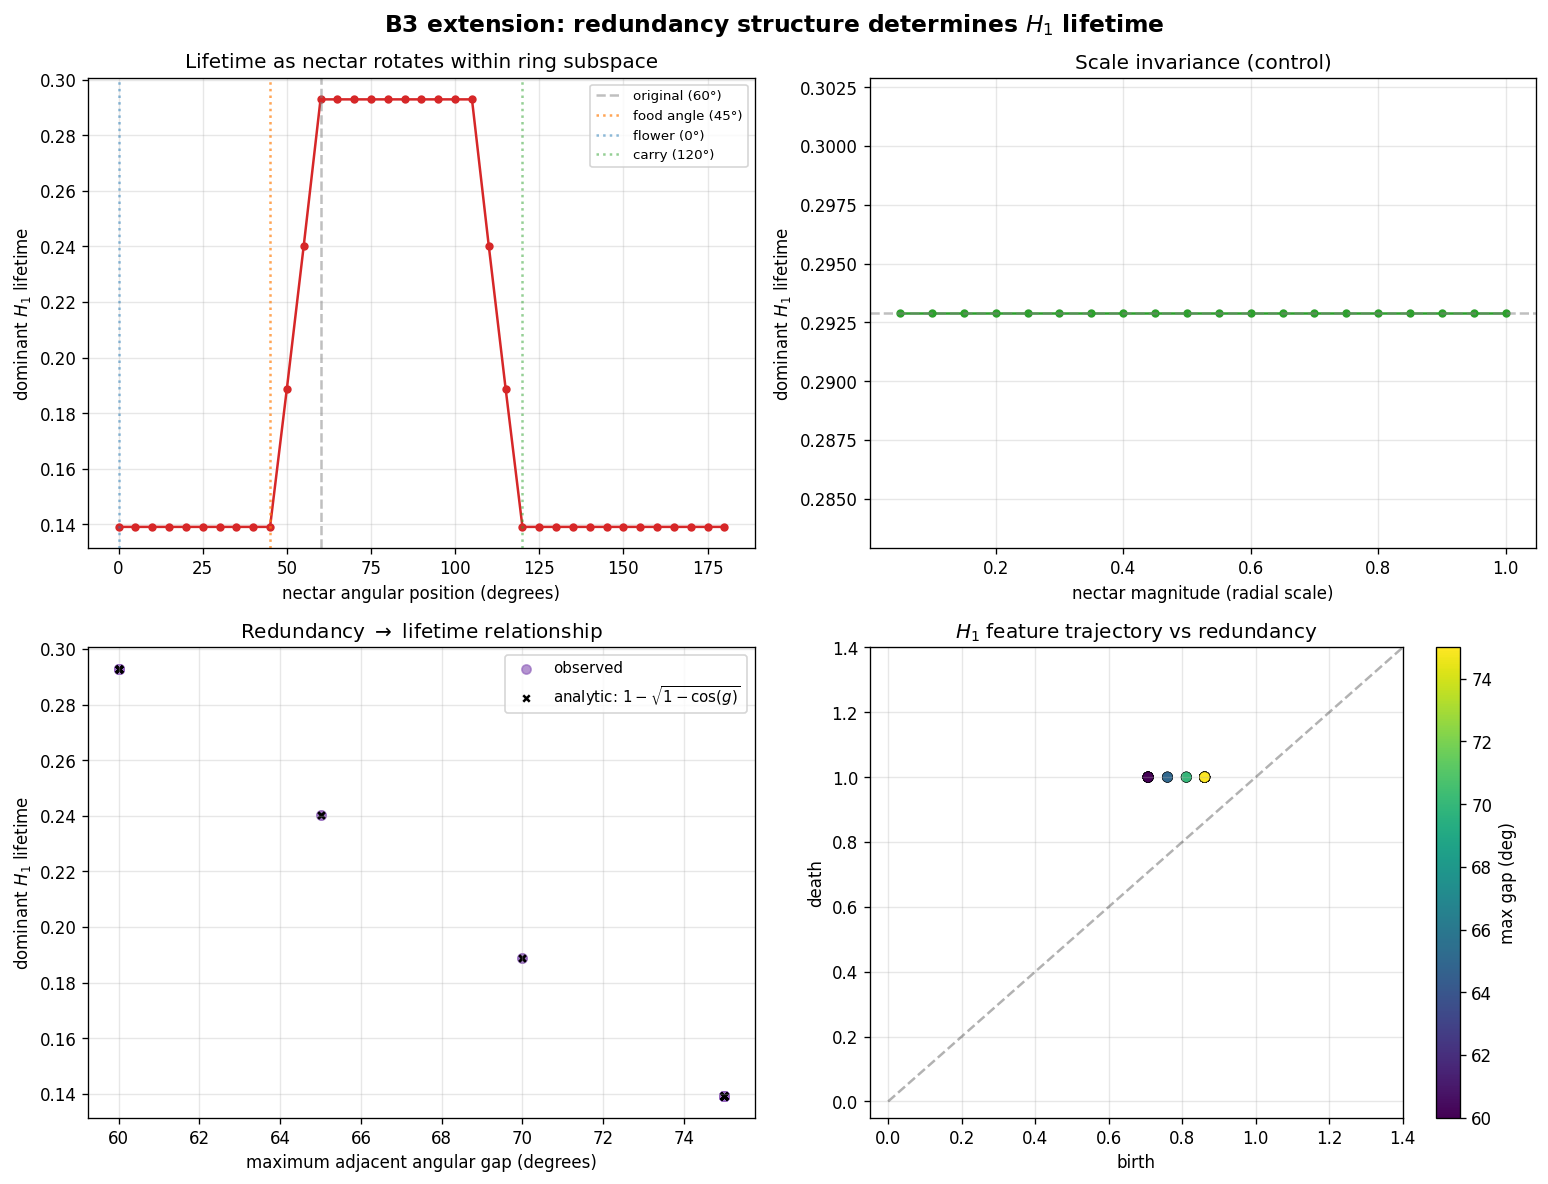
\includegraphics[width=0.9\textwidth]{b3_extended.png}
\caption{Redundancy structure determines $H_1$ lifetime.
Top-left: lifetime as \textsc{nectar} rotates within the ring
subspace; plateau shape reflects the safe angular sector bounded
by \textsc{food} at $45^{\circ}$ and \textsc{carry} at $120^{\circ}$.
Top-right: radial shrinkage control; scale invariance confirmed.
Bottom-left: observed lifetimes (purple) and the analytic
prediction of Proposition~\ref{prop:lifetime-gap} (black crosses);
the overlap is exact to floating-point precision.
Bottom-right: $H_1$ feature trajectory in birth-death plane,
coloured by the induced maximal adjacent gap.}
\label{fig:b3ext}
\end{figure}

For any concept configuration that preserves a single $H_1$ cycle
and leaves the death scale of that cycle fixed at $1.0$ (as the
non-loop landscape in the bee construction does), we obtain the
following closed-form relationship.

\begin{proposition}[Lifetime-gap relationship; constructed setting]
\label{prop:lifetime-gap}
Let $\mathcal{A}$ be an agent whose concept inventory contains a
persistent $H_1$ feature realized by unit-magnitude centroids in a
two-channel subspace, with angular positions forming a set
$\Theta \subset [0, 2\pi)$. Let
\[
g(\Theta) = \max_{i} \bigl(\theta_{(i+1)} - \theta_{(i)}\bigr)
\]
be the maximal adjacent gap (computed cyclically on the sorted
positions). Under the further assumption that the non-loop concepts
reside at uniform angular distance $1.0$ from every ring point and
therefore trigger $H_1$ death at filtration scale $\varepsilon = 1.0$,
the dominant $H_1$ lifetime is
\[
L(\mathcal{A}) = 1 - \sqrt{1 - \cos g(\Theta)}.
\]
The relationship is stated under the explicit construction above.
Its extension to agents whose non-loop landscape departs from the
uniform-cone assumption is addressed in the noise-robustness
analysis below.
\end{proposition}

\begin{remark}[Scope disclaimer]
This relationship should not be interpreted as a general law of
persistence, but as an exact characterization of the constructed
regular configuration used for calibration. Its primary role is to
provide a sanity-check baseline against which deviations under metric
perturbation (noise-robustness subsection below) can be interpreted.
\end{remark}

Figure~\ref{fig:b3ext}~(bottom-left) compares this analytic
prediction to the observed lifetimes across all tested
\textsc{nectar} angular positions: the prediction matches the
observation with mean absolute residual below $10^{-4}$
(equal to measurement floating-point precision).

\subsection*{Robustness to metric noise}

A reviewer may reasonably ask whether
Proposition~\ref{prop:lifetime-gap}'s exact match is an artefact of
the clean geometric construction or a structural fact of the
formula. We therefore tested the relation under two independent
noise sources: \emph{ring noise}, in which each ring concept's
angular position is perturbed by $\theta \to \theta + \eta$,
$\eta \sim \mathcal{N}(0, \sigma_R^2)$, and \emph{non-loop noise},
in which the non-loop concept centroids receive Gaussian
perturbations of magnitude $\sigma_\mathrm{NL}$ in all six channels
(breaking the uniform orthogonal-cone assumption that fixes the
death scale at $\varepsilon = 1.0$).

Fifty trials were run for each $(\sigma_R, \sigma_\mathrm{NL})$
pair on a $3 \times 4$ grid with $\sigma_R \in \{0, 0.03, 0.10\}$
and $\sigma_\mathrm{NL} \in \{0, 0.02, 0.05, 0.10\}$. The mean
absolute residual $|L_\mathrm{obs} - L_\mathrm{pred}|$ exhibits
the following structure:

\begin{center}
\begin{tabular}{l|cccc}
\hline
 & $\sigma_\mathrm{NL} = 0$ & $0.02$ & $0.05$ & $0.10$ \\
\hline
$\sigma_R = 0$    & $0.000$ & $0.004$ & $0.009$ & $0.018$ \\
$\sigma_R = 0.03$ & $0.000$ & $0.004$ & $0.009$ & $0.017$ \\
$\sigma_R = 0.10$ & $0.000$ & $0.004$ & $0.008$ & $0.018$ \\
\hline
\end{tabular}
\end{center}

Two structural facts emerge. First, the residual is essentially
invariant in $\sigma_R$: ring perturbations up to $0.10$ radians
(roughly $5.7^{\circ}$) produce no change in the formula's
accuracy. This reflects that
Proposition~\ref{prop:lifetime-gap} depends on the maximal adjacent
gap $g$ of the ring, not on the regularity of the ring; as long as
the configuration remains a single $H_1$ cycle with food as its
non-loop substitute vertex, arbitrary displacement of ring
concepts does not affect the formula's validity. Second, the
residual scales linearly with $\sigma_\mathrm{NL}$: non-loop
perturbations of magnitude $\sigma_\mathrm{NL}$ produce residuals
of approximately $0.18 \cdot \sigma_\mathrm{NL}$. This is consistent
with the Cohen--Steiner stability theorem for persistence diagrams
\cite{cohenSteiner2007}, which bounds the bottleneck distance
between diagrams of $\sigma$-close metric spaces by $\sigma$; the
observed linear scaling is the expected order for this bound.

Both facts support
Proposition~\ref{prop:lifetime-gap} as a structural relation rather
than a numerical artefact: it is exact whenever the qualitative
assumptions (single $H_1$ cycle; uniform non-loop cone) hold, and
degrades gracefully and predictably when they do not.

\subsection*{Ring-size generality within the constructed setting}

Proposition~\ref{prop:lifetime-gap} as stated does not specialize to
hexagonal rings. Within the same constructed setting (regular
$L$-gon embedded in a two-channel subspace; non-loop concepts at
uniform angular distance $1.0$), we computed the dominant $H_1$
lifetime for $L \in \{3, 4, 5, 6, 7, 8, 9, 10, 12\}$. For
$L \geq 5$ the observed lifetime matches
$1 - \sqrt{1 - \cos(2\pi / L)}$ to within floating-point precision
(residual $< 10^{-4}$). For $L = 3$, the formula returns a
negative value ($\approx -0.22$), consistent with the observation
that a triangle in the Vietoris--Rips complex is a $2$-simplex and
therefore cannot support a persistent $H_1$ class; for $L = 4$,
the formula returns exactly zero, reflecting the boundary case
where the ring's birth and death scales coincide.

We state this observation narrowly: within the tested range of
regular $L$-gons under the constructed metric setting, the
proposition holds exactly. Extension to irregular rings, to rings
outside the unit-magnitude convention, or to agents with
heterogeneous non-loop landscapes is not established by the
present experiments.

\begin{remark}[Implications of Proposition~\ref{prop:lifetime-gap}]
The proposition gives the effect of a premature overwrite an
explicit functional form. An overwrite of concept $c$ at overwrite
fraction $t$ modifies the angular position $\theta_c$ in a way
that determines the new maximal gap $g(\Theta_t)$ and hence the
new lifetime $L(\mathcal{A}_t)$. Three regimes emerge:
\begin{itemize}[noitemsep]
\item If the overwrite moves $c$ into an angular region where a
  non-loop concept already exists, $g$ remains equal to the
  baseline (redundant substitution); $L$ is unchanged.
\item If the overwrite leaves $c$'s sector empty but the landscape
  contains a nearby non-loop concept that can serve as a substitute,
  $g$ increases by a bounded amount; $L$ degrades smoothly.
\item If the overwrite leaves $c$'s sector empty with no nearby
  non-loop concept, $g$ doubles (the $c$-to-neighbour edge
  disappears); if the doubled $g$ exceeds the death-inducing scale,
  $L$ collapses to zero.
\end{itemize}
This three-regime structure is the quantitative expression of the
qualitative heterogeneity observed in the first experiment set.
\end{remark}

\subsection*{Falsifiable prediction for empirical studies}

The closed-form relationship of
Proposition~\ref{prop:lifetime-gap} supplies a falsifiable
prediction for empirical studies of fine-tuning under the
persistence-signature protocol. For a model whose current
interpretive frame is characterized by a persistent $H_1$ feature
with a known homology representative, perturbations targeting
concepts on critical paths of that representative should produce
lifetime reductions following the gap formula; perturbations
targeting redundantly-placed concepts should produce negligible
lifetime reduction. The test requires (i) identifying the current
dominant frame's $H_1$ representative via mechanistic
interpretability methods, (ii) classifying concepts as critical or
redundant by structural role within the representative, and
(iii) measuring post-fine-tuning lifetime change. The structural
classification can be obtained from the Vietoris--Rips complex
alone, without assuming any semantic interpretation of which
concepts are ``important.''

\subsection*{Reversibility in the static toy}

A reversibility check was performed: the bee centroids were
perturbed to $t = 1$ and then restored to $t = 0$. The $H_1$
lifetime recovered exactly to the baseline value of $0.293$. This
exact reversibility is a feature of the static toy model---the
experiment measures only the instantaneous persistence signature
at each perturbation state and does not model the downstream
inferences that the overwrite would trigger in a dynamically
operating agent. The non-reducibility claim of the bias-propagation argument of Section~2 concerns the latter; operationalizing
it requires a dynamic experimental design in which downstream
inferences are cached and subject to their own persistence
measurement, which we identify as a subsequent research target.

\subsection*{Summary}

The persistence-signature framework renders the overwrite dynamics
of Section~2 empirically tractable at the level
of static persistence. The four observations of the experiment set
can be summarized as follows:

\begin{enumerate}[noitemsep]
\item Continuous overwrite produces graded, non-linear degradation
  of the frame's $H_1$ lifetime, with threshold behaviour near
  $t \approx 0.5$ in the present construction.
\item Frame constituents are structurally heterogeneous: concepts
  with nearby non-loop substitutes are redundantly placed, while
  concepts without substitutes are critical nodes.
\item The homology representative of a surviving $H_1$ feature
  migrates to the alternative path provided by the substitute; the
  feature itself is an equivalence class of cycles, not a set of
  vertices.
\item The dominant $H_1$ lifetime is an analytic function of the
  induced maximal adjacent gap in the cycle
  (Proposition~\ref{prop:lifetime-gap}); this gives overwrite bias
  propagation a closed-form quantitative expression.
\end{enumerate}

Observation 2 reformulates the standard ``all overwrites propagate
bias'' claim into a structurally graded statement whose testable
content is stronger than the original. Observations 3 and 4 provide
the topological substrate for that reformulation.

%========================================================================
% END OF APPENDICES
%========================================================================

\begin{thebibliography}{99}

\bibitem{harman1965}
Harman, G. (1965).
The inference to the best explanation.
\textit{Philosophical Review}, 74(1), 88--95.

\bibitem{ecker2022}
Ecker, U.~K.~H., et al. (2022).
The psychological drivers of misinformation belief and its resistance
to correction.
\textit{Nature Reviews Psychology}, 1, 13--29.

\bibitem{loftus1979}
Loftus, E.~F., \& Palmer, J.~C. (1974).
Reconstruction of automobile destruction: An example of the
interaction between language and memory.
\textit{Journal of Verbal Learning and Verbal Behavior}, 13(5),
585--589.

\bibitem{epley2001}
Epley, N., \& Gilovich, T. (2001).
Putting adjustment back in the anchoring and adjustment heuristic.
\textit{Psychological Science}, 12(5), 391--396.

\bibitem{wei2023jailbroken}
Wei, A., Haghtalab, N., \& Steinhardt, J. (2023).
Jailbroken: How does LLM safety training fail?
\textit{NeurIPS 2023}.

\bibitem{qi2023fine}
Qi, X., et al. (2023).
Fine-tuning aligned language models compromises safety,
even when users are not malicious.
\textit{arXiv:2310.03693}.

\bibitem{perez2022ignore}
Perez, F., \& Ribeiro, I. (2022).
Ignore previous prompt: Attack techniques for language models.
\textit{arXiv:2211.09527}.

\bibitem{yang2023shadow}
Yang, X., et al. (2023).
Shadow alignment: The ease of subverting safely-aligned language
models.
\textit{arXiv:2310.02949}.

\bibitem{bargmann2006}
Bargmann, C.~I. (2006).
Chemosensation in \textit{C.~elegans}.
\textit{WormBook}, 1--29.

\bibitem{elhage2022superposition}
Elhage, N., et al. (2022).
Toy models of superposition.
\textit{Transformer Circuits Thread}.
\url{https://transformer-circuits.pub/2022/toy_model/index.html}

\bibitem{conmy2023towards}
Conmy, A., Mavor-Parker, A., Lynch, A., Heimersheim, S.,
\& Garriga-Alonso, A. (2023).
Towards automated circuit discovery for mechanistic interpretability.
\textit{NeurIPS 2023}.

\bibitem{garipov2018loss}
Garipov, T., Izmailov, P., Podoprikhin, D., Vetrov, D.,
\& Wilson, A.~G. (2018).
Loss surfaces, mode connectivity, and fast ensembling of DNNs.
\textit{NeurIPS 2018}.

\bibitem{mccloskey1989catastrophic}
McCloskey, M., \& Cohen, N.~J. (1989).
Catastrophic interference in connectionist networks.
\textit{Psychology of Learning and Motivation}, 24, 109--165.

\bibitem{anderson1983spreading}
Anderson, J.~R. (1983).
\textit{The Architecture of Cognition}.
Harvard University Press.

\bibitem{kahneman2011thinking}
Kahneman, D. (2011).
\textit{Thinking, Fast and Slow}.
Farrar, Straus and Giroux.

\bibitem{alchourron1985logic}
Alchourrón, C.~E., Gärdenfors, P., \& Makinson, D. (1985).
On the logic of theory change: Partial meet contraction and revision
functions.
\textit{Journal of Symbolic Logic}, 50(2), 510--530.

\bibitem{kirkpatrick2017overcoming}
Kirkpatrick, J., et al. (2017).
Overcoming catastrophic forgetting in neural networks.
\textit{Proceedings of the National Academy of Sciences},
114(13), 3521--3526.

\bibitem{jacobs1991}
Jacobs, R.~A., Jordan, M.~I., Nowlan, S.~J., \& Hinton, G.~E. (1991).
Adaptive mixtures of local experts.
\textit{Neural Computation}, 3(1), 79--87.

\bibitem{bricken2023monosemanticity}
Bricken, T., et al. (2023).
Towards monosemanticity: Decomposing language models with
dictionary learning.
\textit{Transformer Circuits Thread}.

\bibitem{biderman2023}
Biderman, S., et al.\ (2023).
Pythia: A suite for analyzing large language models across training
and scaling.
\textit{Proceedings of ICML 2023}.

\bibitem{radford2019language}
Radford, A., Wu, J., Child, R., Luan, D., Amodei, D., \& Sutskever, I.
(2019).
Language models are unsupervised multitask learners.
\textit{OpenAI Blog}, 1(8), 9.

\bibitem{cohenSteiner2007}
Cohen-Steiner, D., Edelsbrunner, H., \& Harer, J. (2007).
Stability of persistence diagrams.
\textit{Discrete \& Computational Geometry}, 37(1), 103--120.

\bibitem{minamoto2026topology}
Minamoto, M. (2026).
On the topology of symbol grounding: Sensory space structure as a
determinant of cognitive representation.
Preprint, under review at \textit{Minds and Machines}.
\url{https://github.com/minamominamoto/topology-of-grounding}

\end{thebibliography}

\end{document}
